\section{Ejercicio: Aprendizaje de distribución en forma geométrica}

Se implementó una red de Kohonen de grilla $10 \times 10$ con 2 entradas. Los pesos se inicializan aleatoriamente en $[-1,1]^2$ y se entrenan durante 10.000 iteraciones usando una función de vecindad gaussiana con radio $\sigma$ decreciente. En cada figura se muestran snapshots del mapa en distintas iteraciones: los puntos grises son las muestras de entrenamiento, los nodos rojos son los pesos de las neuronas y las líneas azules conectan neuronas vecinas en la grilla.

\subsection{Círculo unitario}

En la figura~\ref{fig:circulo} se puede observar cómo la grilla se despliega desde una distribución inicial desordenada hasta adaptarse a la forma circular, cubriendo el disco de manera uniforme y preservando la vecindad entre neuronas.

\begin{figure}[htbp]
    \centering
    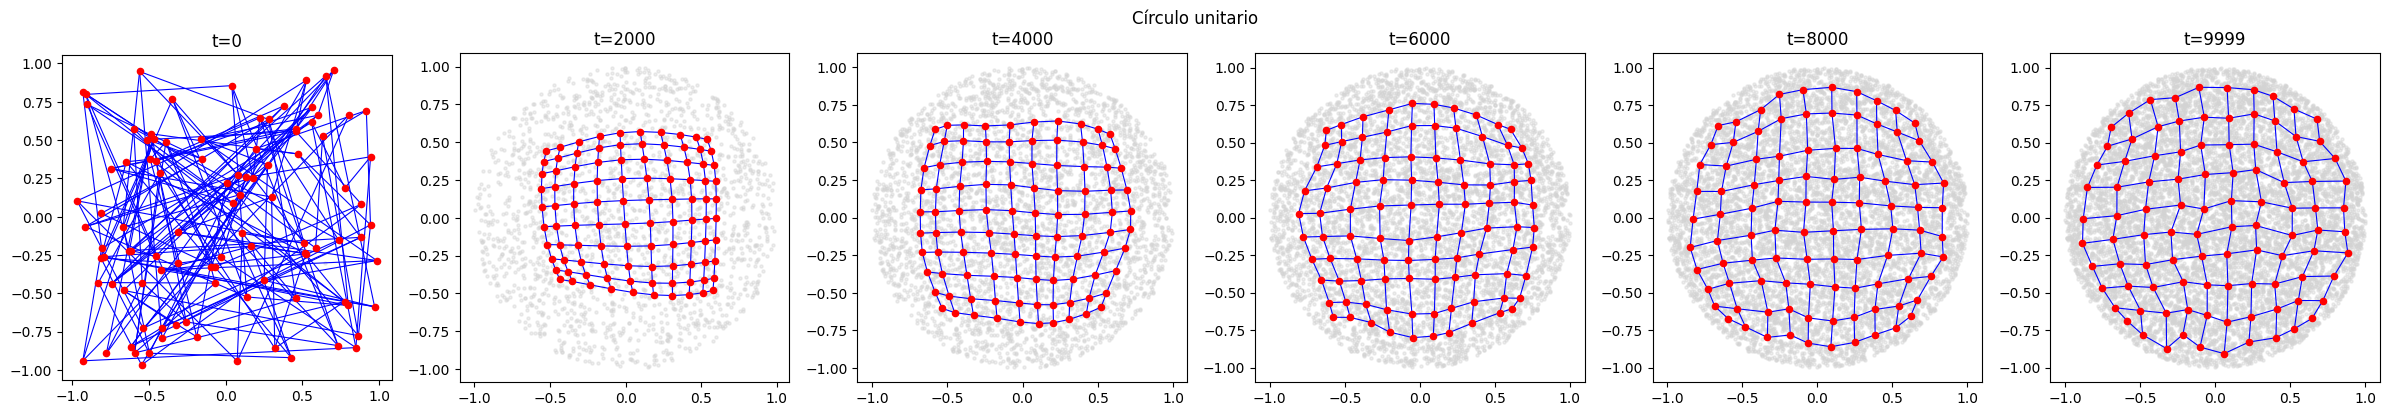
\includegraphics[width=\textwidth]{img_informe/ej1/circulo_unitario}
    \caption{Evolución del mapa entrenado sobre el círculo unitario.}
    \label{fig:circulo}
\end{figure}

\subsection{Cuadrado}

En la figura~\ref{fig:cuadrado} se puede observar que el cuadrado es la figura más compatible con la topología de una grilla rectangular: el mapa converge rápidamente sin cruces ni pliegues, cubriendo de forma uniforme toda la región.

\begin{figure}[htbp]
    \centering
    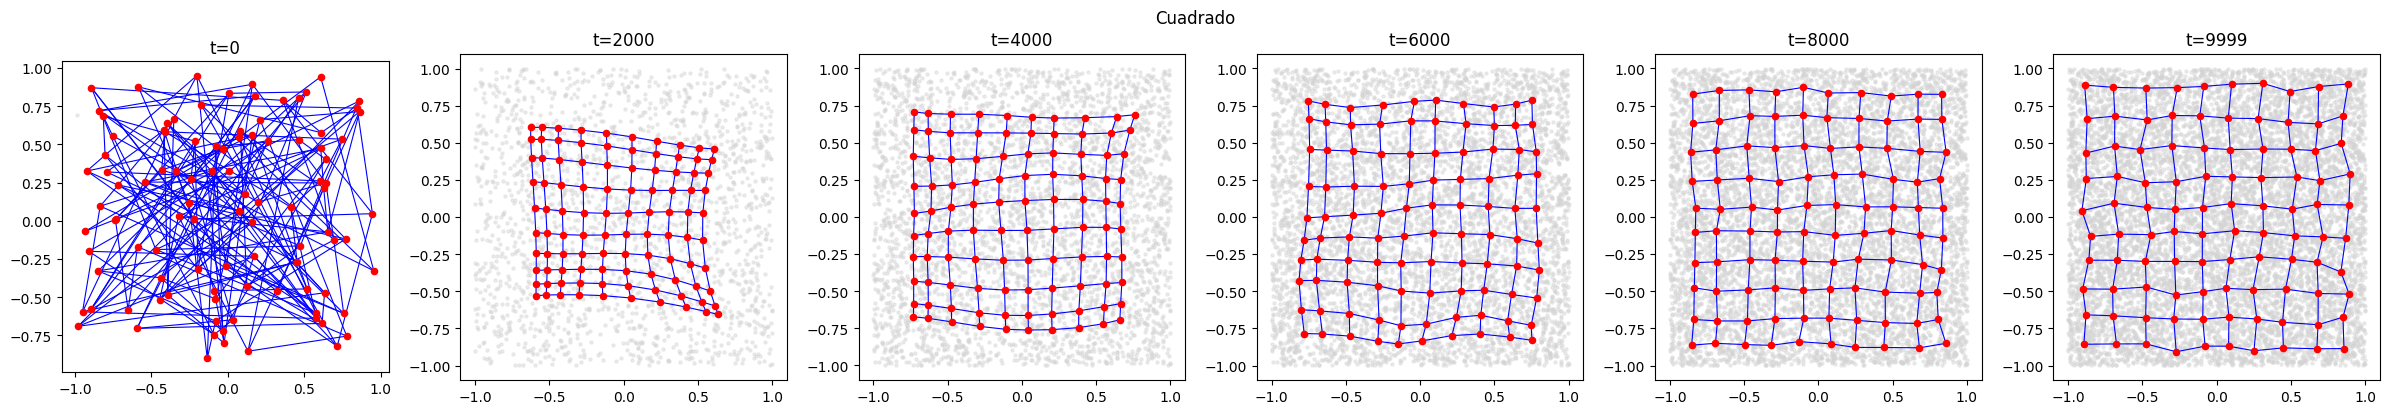
\includegraphics[width=\textwidth]{img_informe/ej1/cuadrado}
    \caption{Evolución del mapa entrenado sobre el cuadrado $[-1,1]^2$.}
    \label{fig:cuadrado}
\end{figure}

\subsection{Triángulo}

En la figura~\ref{fig:triangulo} se puede observar que la red logra adaptarse a la forma triangular, aunque la incompatibilidad entre la grilla cuadrada y la geometría triangular genera cierta distorsión en las esquinas, donde algunas neuronas quedan comprimidas.

\begin{figure}[htbp]
    \centering
    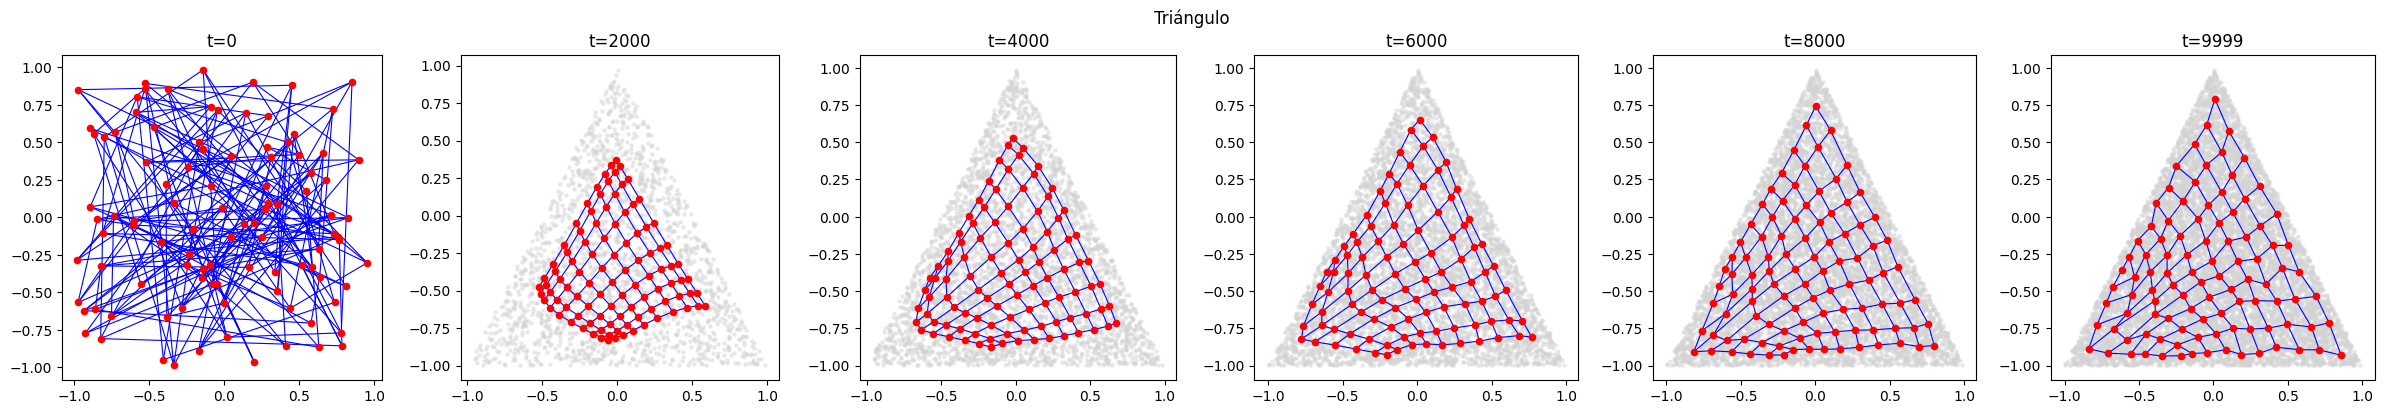
\includegraphics[width=\textwidth]{img_informe/ej1/triangulo}
    \caption{Evolución del mapa entrenado sobre el triángulo.}
    \label{fig:triangulo}
\end{figure}

\subsection{Anillo}

En la figura~\ref{fig:anillo} se puede observar que el anillo es topológicamente incompatible con una grilla plana: para cubrirlo, la grilla necesitaría cerrarse sobre sí misma. El resultado final muestra pliegues o cruces inevitables en algún punto del mapa.

\begin{figure}[htbp]
    \centering
    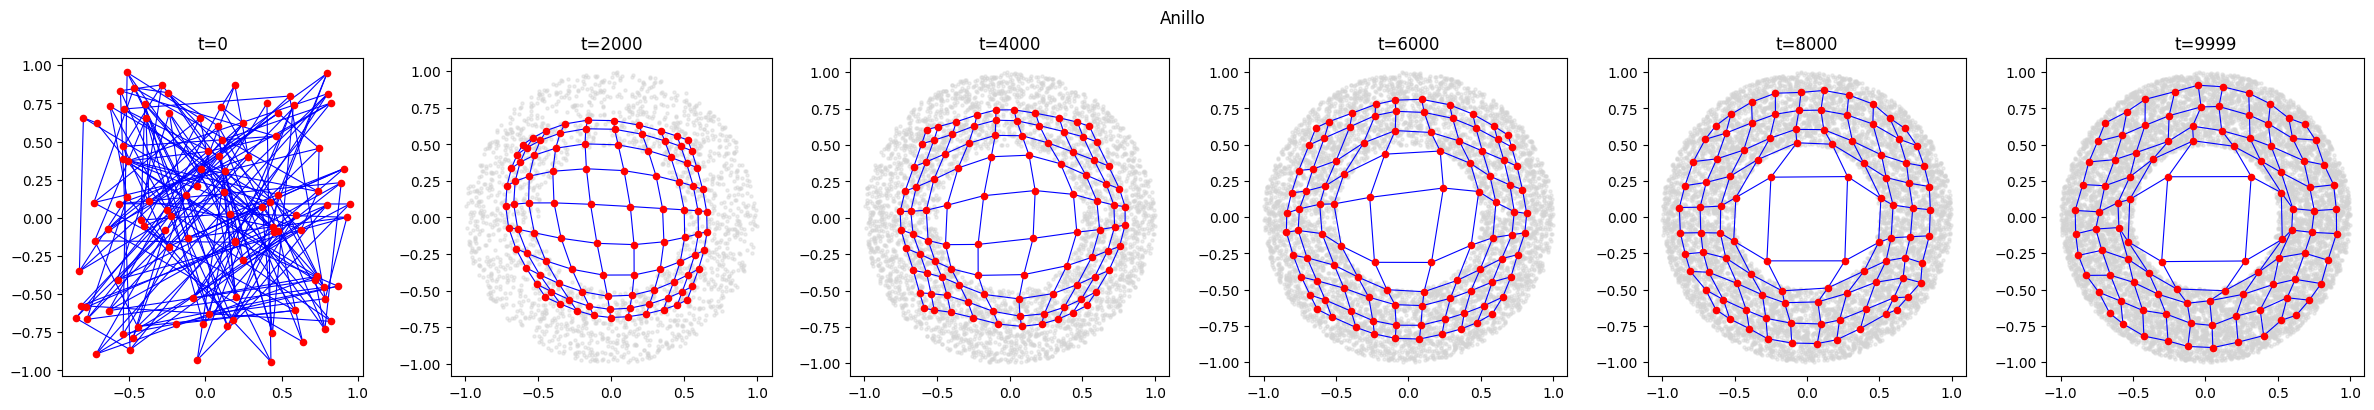
\includegraphics[width=\textwidth]{img_informe/ej1/anillo}
    \caption{Evolución del mapa entrenado sobre un anillo ($r \in [0.5, 1.0]$).}
    \label{fig:anillo}
\end{figure}

\subsection{Dos anillos concéntricos}

En la figura~\ref{fig:anillo_disco} se puede observar que la distribución, al tener dos regiones separadas por una zona vacía, genera tensión topológica en el mapa: la grilla se divide entre ambas regiones y se forman pliegues en la zona de transición.

\begin{figure}[htbp]
    \centering
    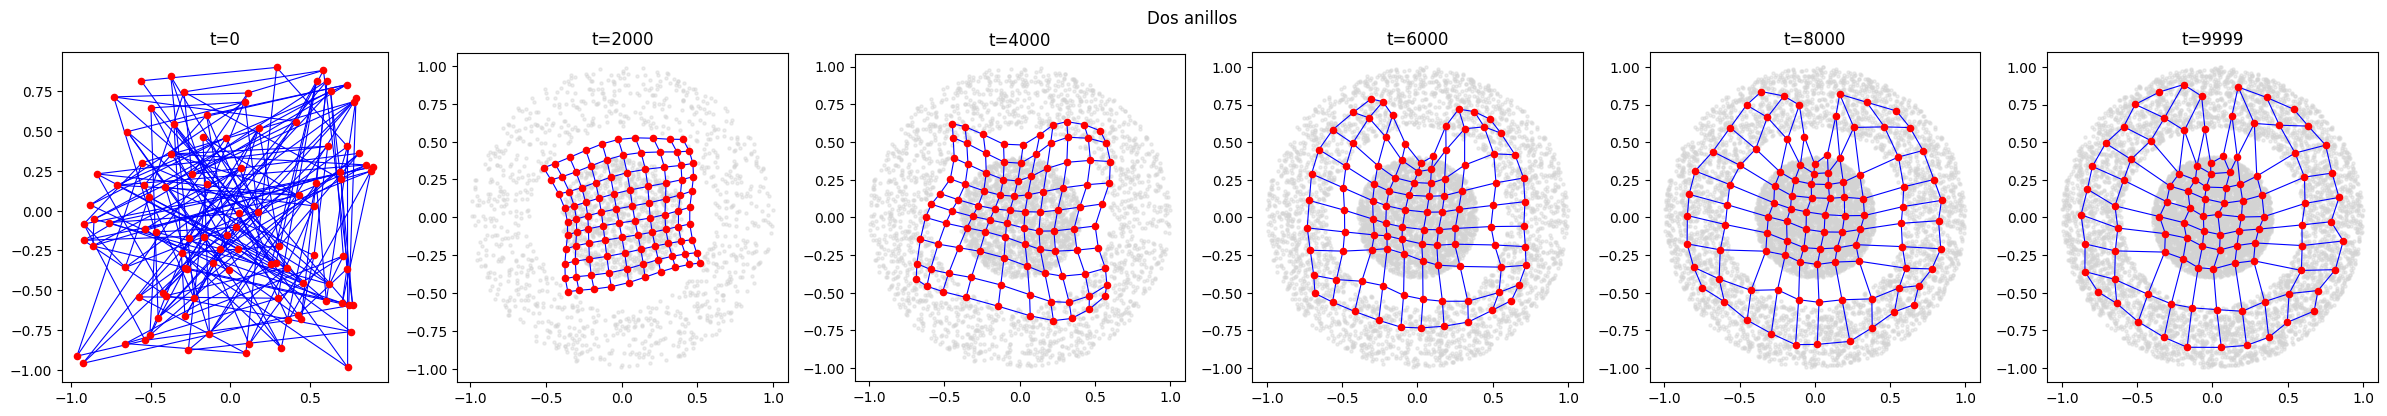
\includegraphics[width=\textwidth]{img_informe/ej1/anillo_disco}
    \caption{Evolución del mapa entrenado sobre dos anillos concéntricos.}
    \label{fig:anillo_disco}
\end{figure}

\subsection{Dos clusters gaussianos}

En la figura~\ref{fig:clusters} se puede observar que el mapa asigna grupos de neuronas a cada cluster, con la separación entre ambos claramente reflejada en la organización de la grilla.

\begin{figure}[htbp]
    \centering
    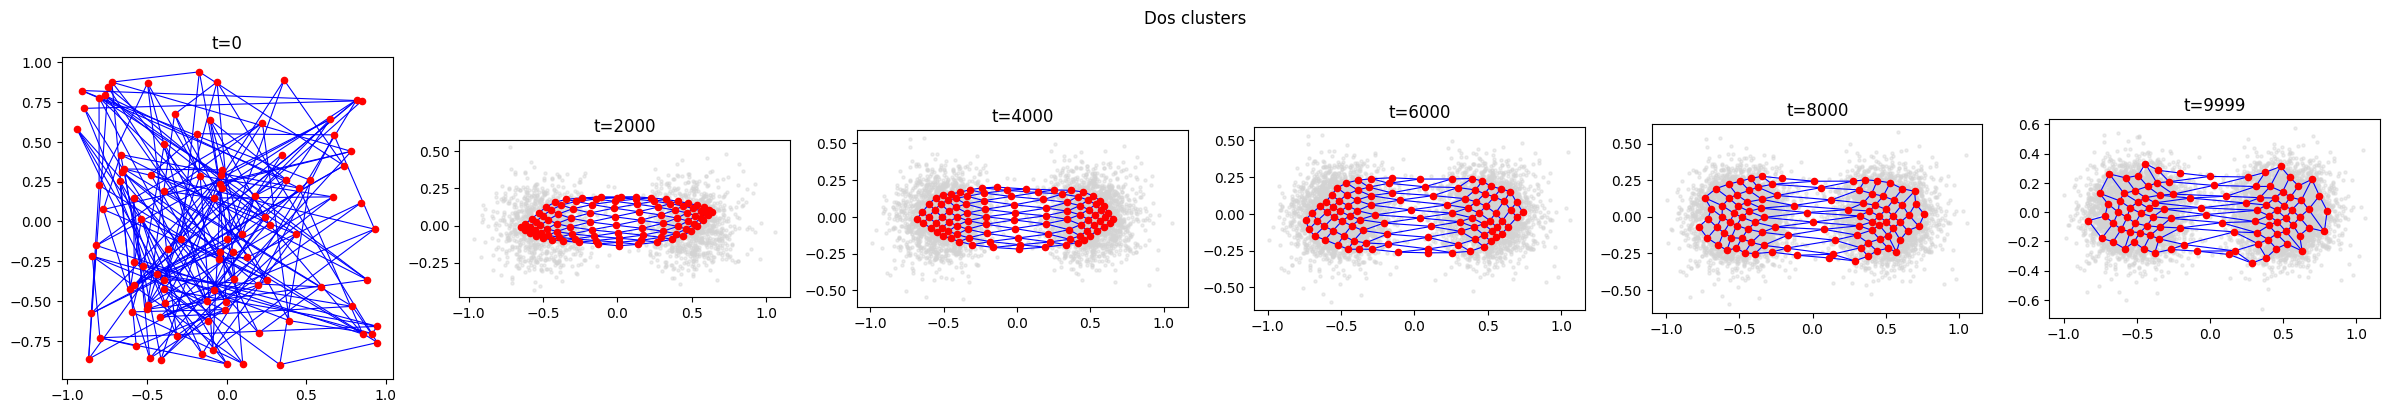
\includegraphics[width=\textwidth]{img_informe/ej1/dos_clusters}
    \caption{Evolución del mapa entrenado sobre dos clusters gaussianos.}
    \label{fig:clusters}
\end{figure}

\subsection{Letra M}

En la figura~\ref{fig:M} se puede observar que la estructura ramificada de la letra M no puede representarse sin cruces con una grilla plana. El mapa logra adaptarse a los trazos principales, aunque aparecen pliegues en las zonas donde los segmentos se unen.

\begin{figure}[htbp]
    \centering
    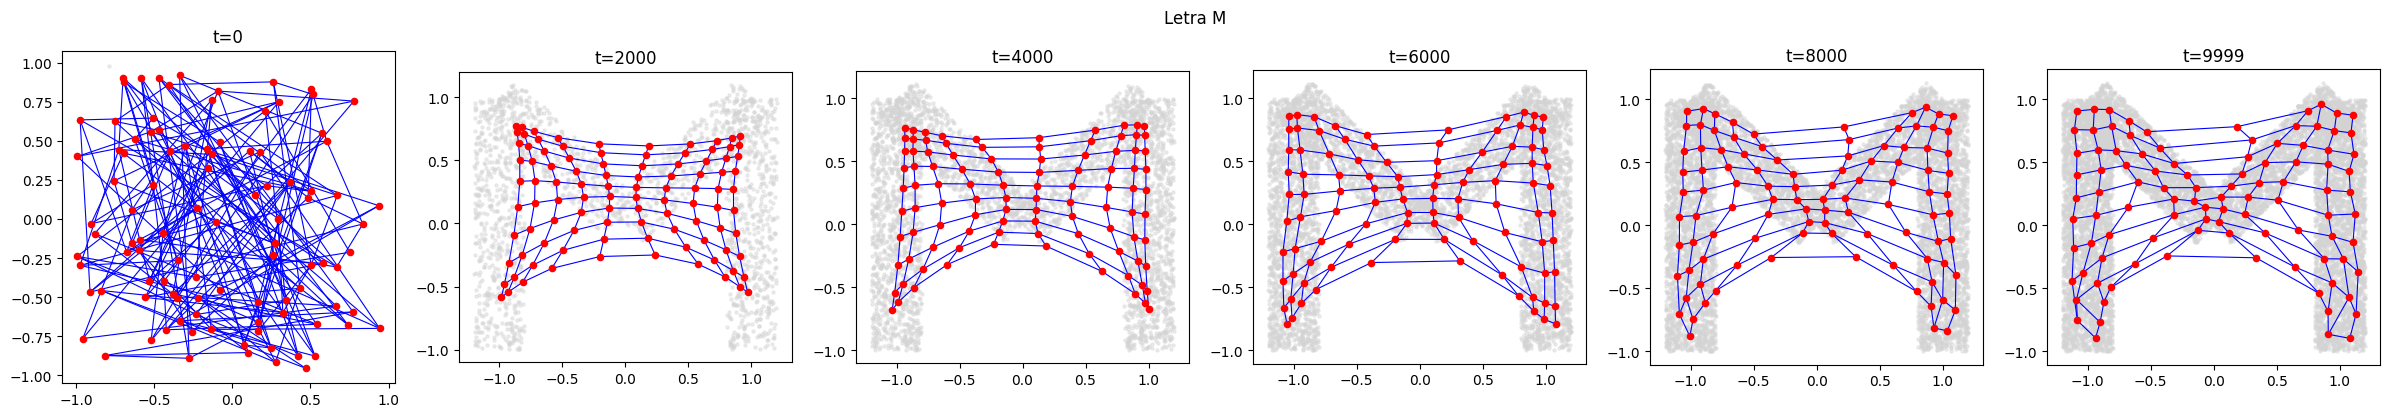
\includegraphics[width=\textwidth]{img_informe/ej1/M}
    \caption{Evolución del mapa entrenado sobre la figura de la letra M.}
    \label{fig:M}
\end{figure}

\section{Ejercicio 2: Travelling Salesman Problem}


El \textit{Traveling Salesman Problem} (TSP) consiste en encontrar el tour de mínima longitud que visite exactamente una vez cada una de las $N$ ciudades y regrese al punto de partida. El problema es NP-hard, por lo que en la práctica se buscan soluciones aproximadas.

La diferencia clave respecto al ejercicio anterior es la topología de la red: en lugar de una grilla 2D, se usa un \textbf{anillo 1D} de $M$ neuronas (con $M > N$). El orden de las neuronas en el anillo define directamente el orden de visita del tour. Las neuronas se inicializan en un pequeño círculo centrado en el centroide de las ciudades.

La distancia entre dos neuronas $i$ y $j$ en el anillo es circular:

\begin{equation}
	d_{\text{ring}}(i,\,j) = \min\!\left(|i - j|,\; M - |i - j|\right)
\end{equation}

lo que garantiza que la vecindad se envuelva al llegar al extremo del anillo.

En cada época se presentan todas las ciudades. Para cada ciudad $\bar{x}$, se encuentra la neurona ganadora $i^*$ (la más cercana en espacio euclídeo) y se actualizan los pesos con la misma regla que en el ejercicio 1, pero usando $d_{\text{ring}}$ en la función de vecindad gaussiana.

Se experimentó con distintos valores del factor $M/N \in \{1, 2, 3\}$. Tener más neuronas que ciudades permite una mejor cobertura del espacio pero aumenta el costo computacional. La calidad de la solución se evalúa con la longitud total del tour.

\subsection{$M/N = 1$}

Como primer intento se utilizó un factor $M/N = 1$, para ver si con una neurona por ciudad era suficiente. En la figura~\ref{fig:evolucion_1} se observa como la red aprende paulatinamente y se adapta a un recorrido que abarca cada una de las ciudades. Empieza como un circulo pequeño y alrededor de la epoca 49 ya se agranda, cubriendo el terreno de todas las ciudades. 

Al finalizar el entrenamiento, como se observa en la figura~\ref{fig:camino_1}, la red logra trazar un recorrido cerrado que cubre la región de las ciudades. Sin embargo, con $M/N = 1$ el anillo no tiene suficiente resolución para adaptarse a todas ellas: el camino formado por los pesos de las neuronas no logra exactamente por todas las ciudades. Se aumentó el número de épocas de entrenamiento, pero aun así el resultado no mejoró significativamente. Se concluye que un factor $M/N = 1$ es insuficiente para obtener una solución de calidad.

\begin{figure}[htbp]
	\centering
	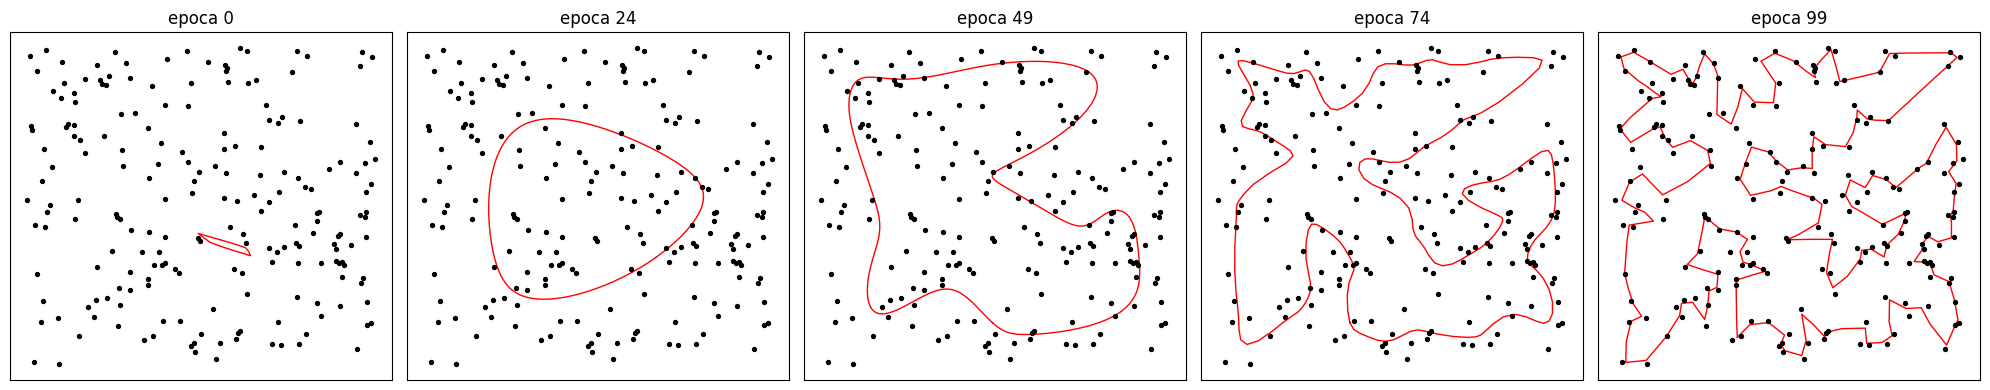
\includegraphics[width=\textwidth]{img_informe/ej2/evolucion_1.png}
	\caption{Evolución del anillo entrenado sobre el conjunto de ciudades.}
	\label{fig:evolucion_1}
\end{figure}

\begin{figure}[htbp]
	\centering
	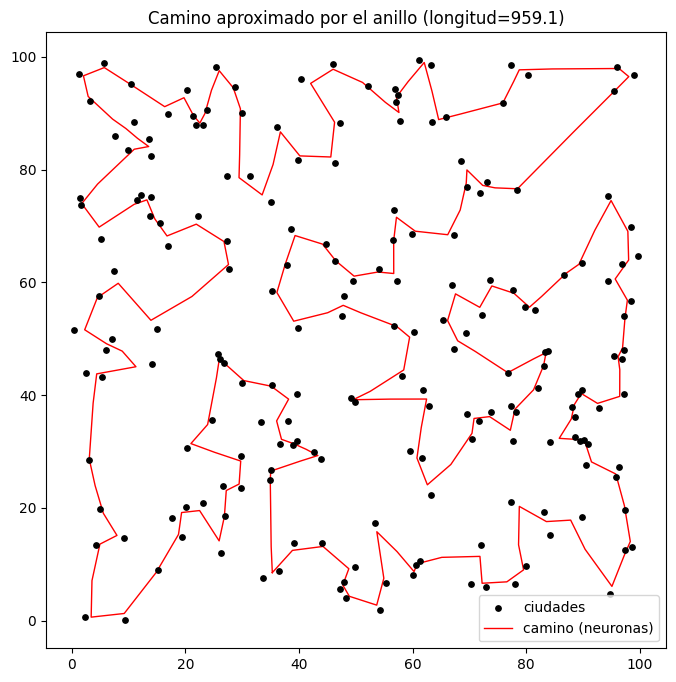
\includegraphics[width=0.6\textwidth]{img_informe/ej2/camino_1.png}
	\caption{Resolución de la red para $M/N = 1$.}
	\label{fig:camino_1}
\end{figure}

\subsection{$M/N = 2$}

Para la segunda prueba se incrementó la cantidad de neuronas por ciudad al doble. En la figura~\ref{fig:evolucion_2} se puede observar el proceso de aprendizaje y en la figura~\ref{fig:camino_2} el camino final trazado por las neuronas.

Se puede observar como en este caso las neuronas logran pasar directamente por casi todas las ciudades. Vale la pena notar que los pliegues extra que se requieren para lograr esto hacen que el camino sea más largo.

\begin{figure}[htbp]
	\centering
	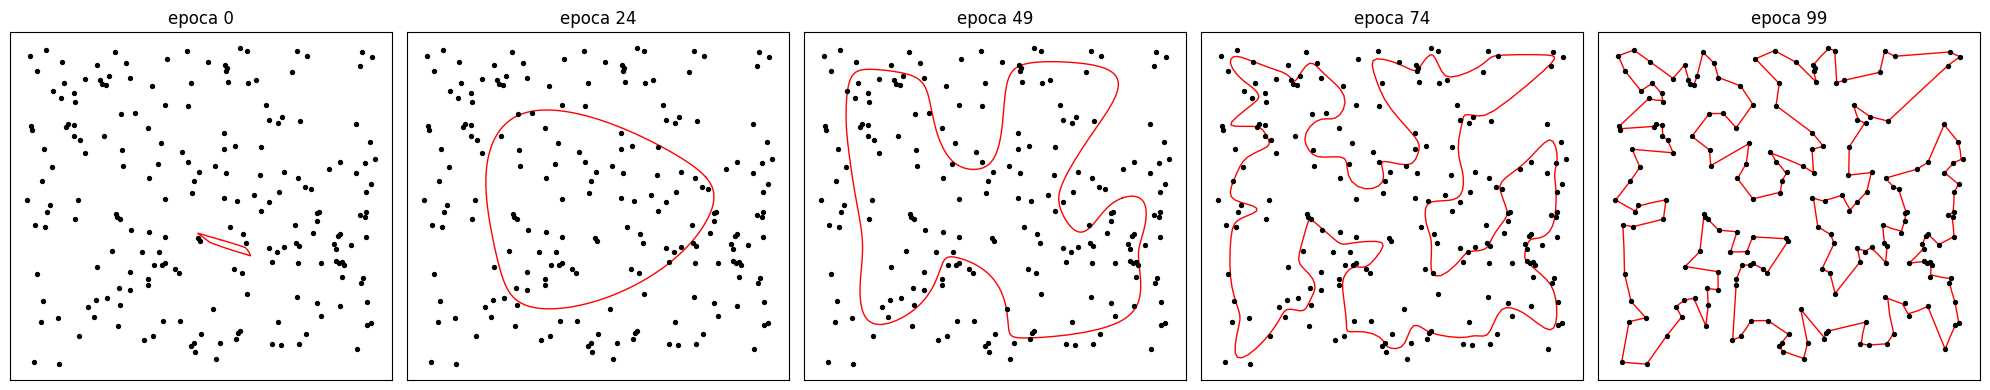
\includegraphics[width=\textwidth]{img_informe/ej2/evolucion_2.png}
	\caption{Evolución del anillo entrenado sobre el conjunto de ciudades.}
	\label{fig:evolucion_2}
\end{figure}

\begin{figure}[htbp]
	\centering
	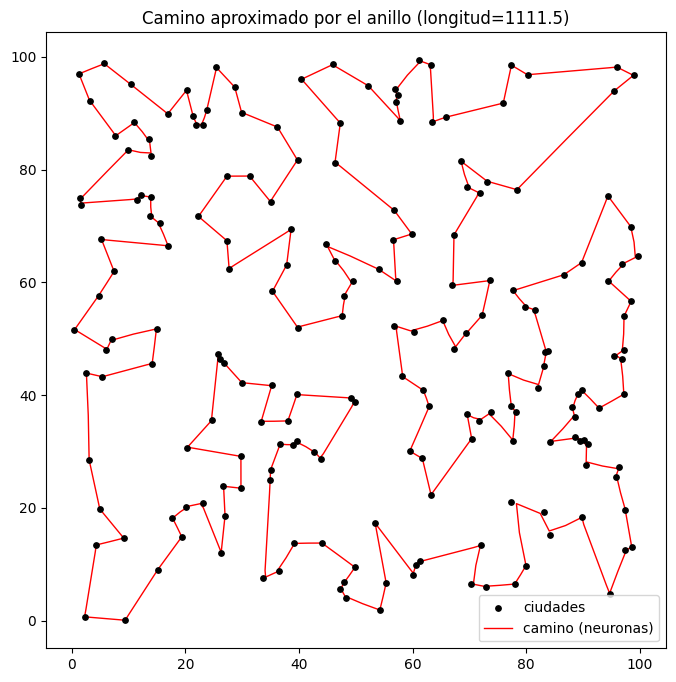
\includegraphics[width=0.6\textwidth]{img_informe/ej2/camino_2.png}
	\caption{Resolución de la red para $M/N = 2$.}
	\label{fig:camino_2}
\end{figure}

\subsection{$M/N = 3$}

Para el útlimo caso, se aumentó una vez más la relación neurona/ciudad. La figuras~\ref{fig:evolucion_3} y~\ref{fig:camino_3} muestran el resultado. Se observa una leve mejora respecto del caso anterior. Ahora si todas las ciudades son cubiertas por el recorrido, haciendo el camino sea un poco más largo.

\begin{figure}[htbp]
	\centering
	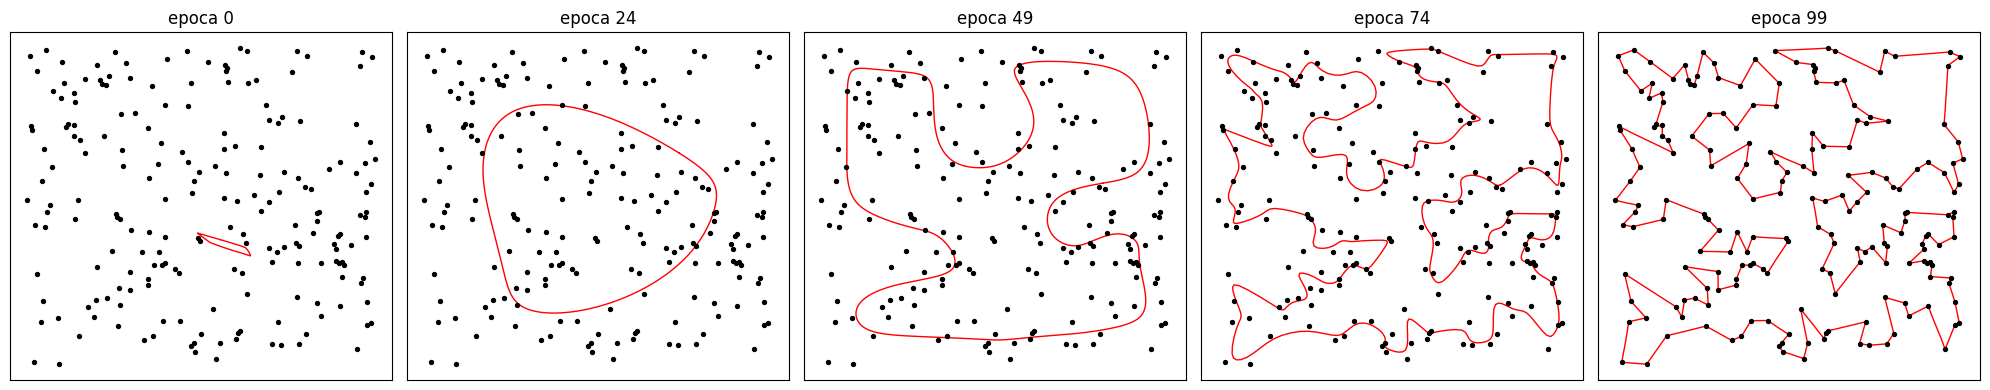
\includegraphics[width=\textwidth]{img_informe/ej2/evolucion_3.png}
	\caption{Evolución del anillo entrenado sobre el conjunto de ciudades.}
	\label{fig:evolucion_3}
\end{figure}

\begin{figure}[htbp]
	\centering
	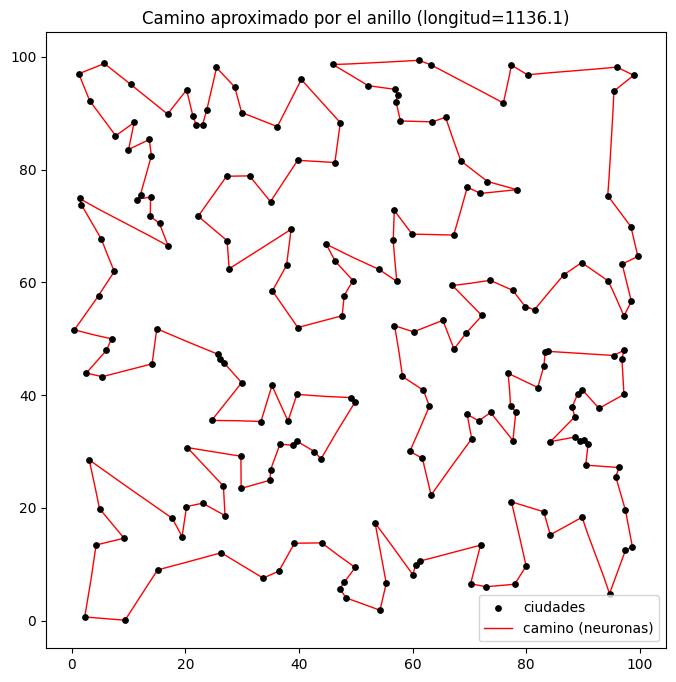
\includegraphics[width=0.6\textwidth]{img_informe/ej2/camino_3.png}
	\caption{Resolución de la red para $M/N = 3$.}
	\label{fig:camino_3}
\end{figure}

Entonces se puede concluir, que a fines prácticos, la red de Kohonen hace un buen trabajo para encontrar una aproximación del camino ideal. El factor $M/N = 2$ hizo un trabajo lo suficientemente bueno como para poder apreciar el orden de visita de las ciudades.


\section{Ejercicio 3: Reducción de dimensionalidad y clustering}

Los datos consisten en 500 muestras de una variable de 100 dimensiones. El objetivo es reducir la dimensionalidad y detectar la presencia de clusters.

La reducción de dimensionalidad surge de forma natural al entrenar una SOM sobre datos de alta dimensión: cada neurona de la grilla 2D aprende a representar una región del espacio de 100 dimensiones, de modo que cualquier muestra puede mapearse a la posición 2D de su BMU. Así, el entrenamiento transforma implícitamente cada vector de $\mathbb{R}^{100}$ en una coordenada $(i, j)$ de la grilla, pasando de 100 dimensiones a 2 sin necesidad de ningún paso adicional.

Para detectar clusters se utiliza la \textbf{matriz U} (\textit{Unified Distance Matrix}): para cada neurona se calcula la distancia promedio a sus vecinas en la grilla. Zonas con distancias bajas (neuronas similares entre sí) corresponden a regiones densas del espacio de entrada, mientras que zonas con distancias altas indican fronteras entre clusters.

En la figura~\ref{fig:U} se observa como los colores oscuros representan las zonas densas, indicando la presencia de clusters. Por otro lado, las zonas claras evidencian alta distancia entre neuronas vecinas, lo cual significa separación de clusters. Se pueden identificar 5 clusters facilmente.


\begin{figure}[htbp]
	\centering
	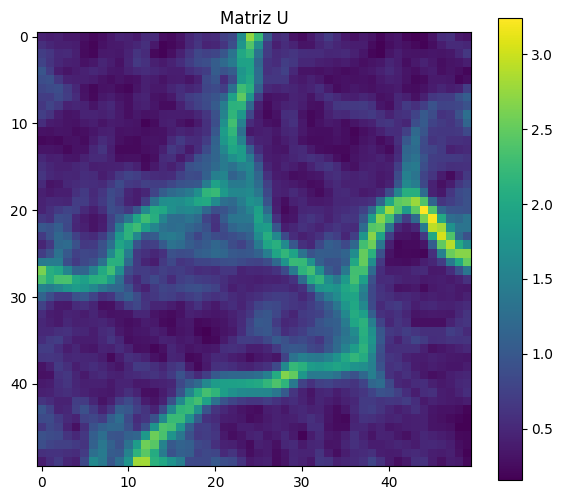
\includegraphics[width=0.6\textwidth]{img_informe/ej3/matriz_U.png}
	\caption{Matriz U con código de colores para poder identidicar clusters.}
	\label{fig:U}
\end{figure}

